\section{Experimental Setup}
\label{sec:experiments}

\subsection{Dataset Selection and Profiling}
We evaluate our approach on the \textbf{DS2OS} (Distributed Smart Space Orchestration System) dataset~\cite{shivanjali2020ensemble}, which is one of the two primary datasets benchmarked in the DIFT paper~\cite{wang2025dift}. DS2OS was gathered in an IoT smart home testbed containing real and simulated smart devices (thermostats, door locks, cameras, environmental monitors) communicating over HTTP and MQTT protocols.

The dataset contains 357,952 connection traces across eight categories: one benign class and seven attack types. As shown in Fig.~\ref{fig:class_dist}, the dataset has extreme class imbalance:
\begin{itemize}
    \item \textbf{Normal:} 347,935 samples (97.20\% of total).
    \item \textbf{DoS:} 5,780 samples (1.615\%, ratio 60:1).
    \item \textbf{Scan:} 1,547 samples (0.432\%, ratio 225:1).
    \item \textbf{Malicious Control:} 889 samples (0.248\%, ratio 391:1).
    \item \textbf{Malicious Operation:} 805 samples (0.225\%, ratio 432:1).
    \item \textbf{Spying:} 532 samples (0.149\%, ratio 654:1).
    \item \textbf{Data Probing:} 342 samples (0.096\%, ratio 1,017:1).
    \item \textbf{Wrong Setup:} 122 samples (0.034\%, ratio 2,851:1).
\end{itemize}

\begin{figure*}[!t]
\centering
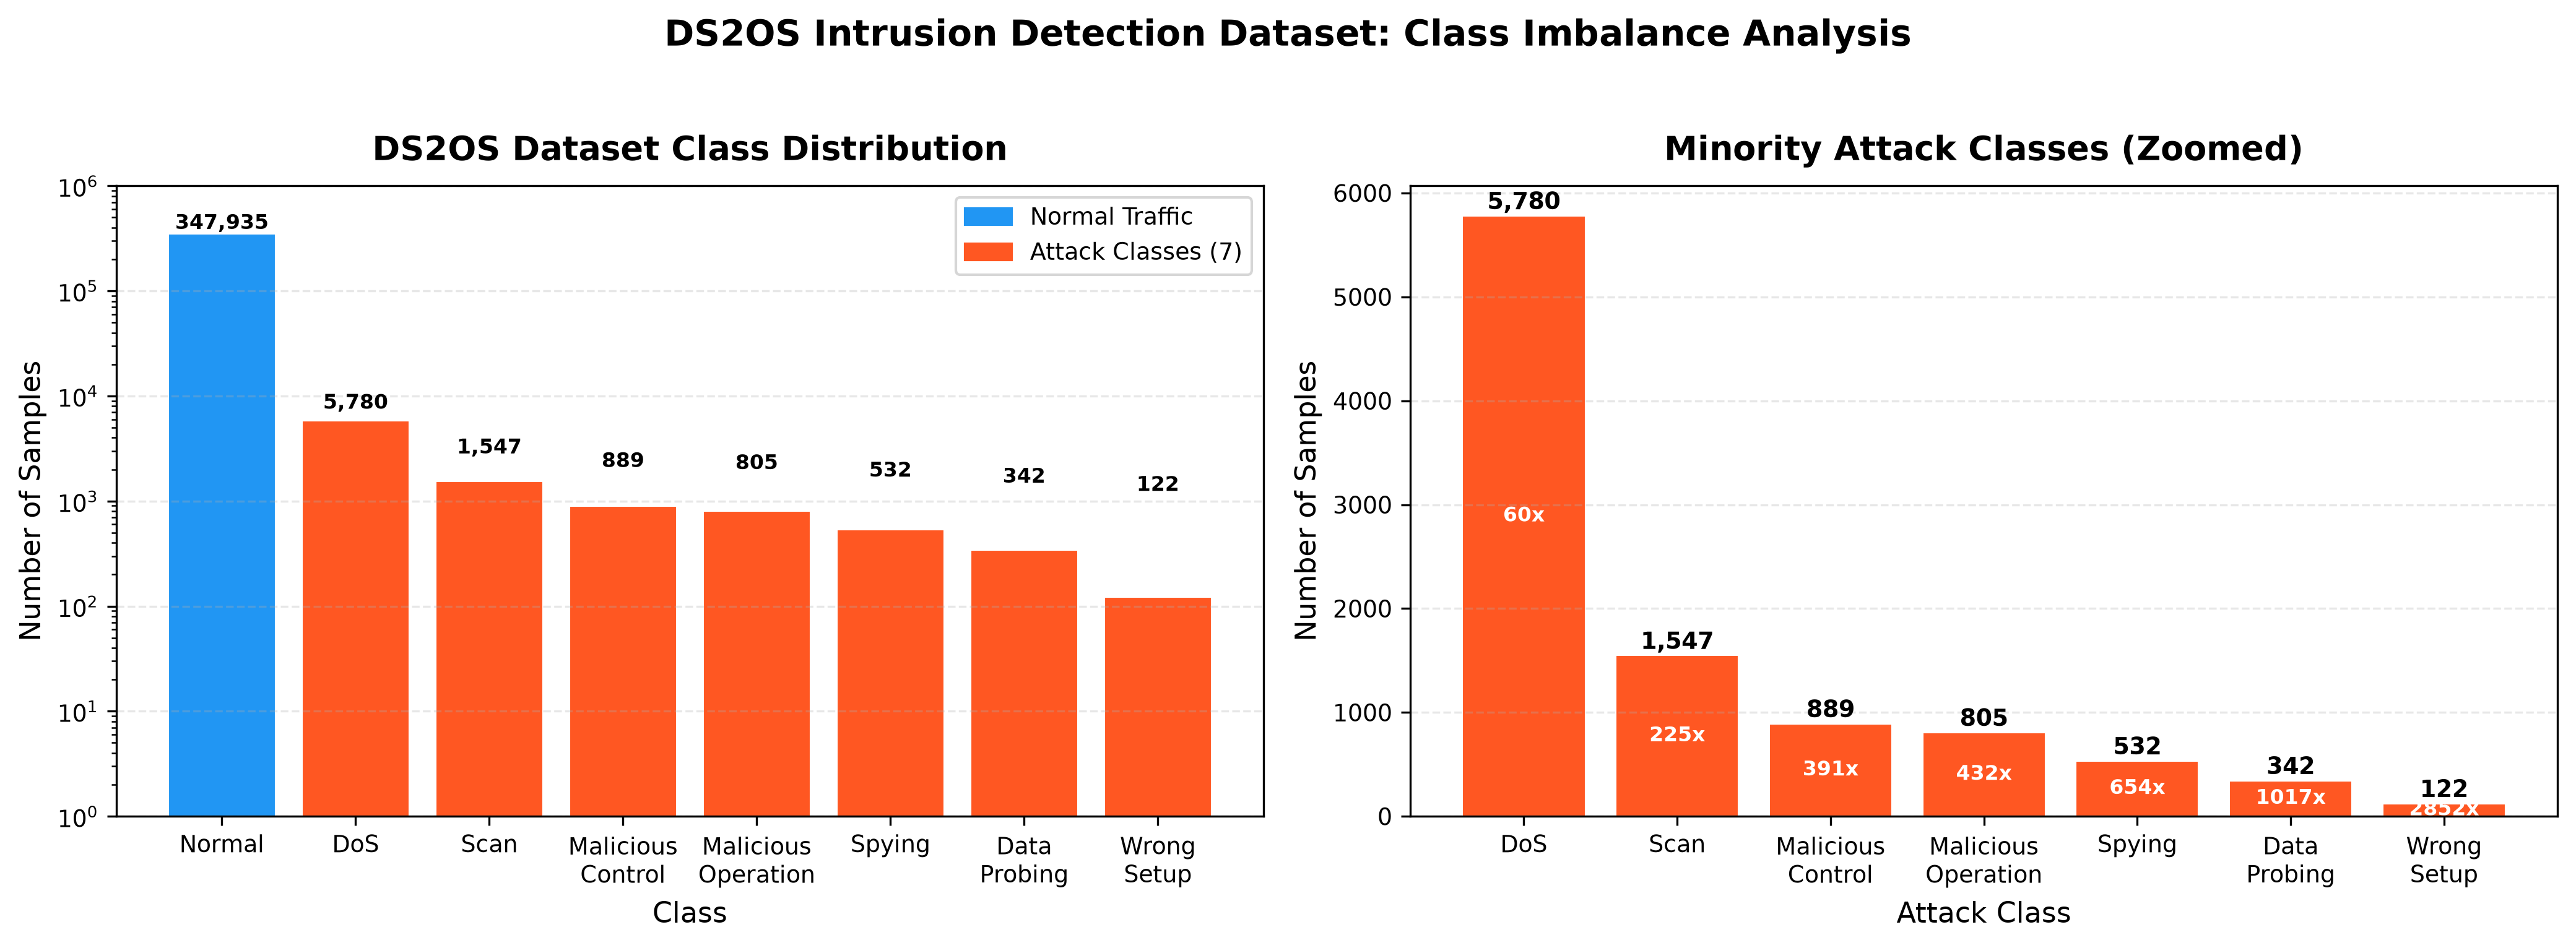
\includegraphics[width=0.92\textwidth]{images/1.png}
\caption{DS2OS dataset class distribution shown on a logarithmic scale (left) and detailed minority attack sample counts with imbalance ratios relative to benign traffic (right).}
\label{fig:class_dist}
\end{figure*}

\subsection{Preprocessing and Data Cleaning}
The raw dataset contains 13 attributes per trace. We immediately drop five identifier columns that do not generalize across networks: \texttt{sourceid}, \texttt{sourceAddress}, \texttt{destinationServiceAddress}, \texttt{accessedNodeAddress}, and \texttt{timestamp}. 

For the remaining seven attributes:
\begin{itemize}
    \item \texttt{accessedNodeType} has missing values in roughly 15\% of rows; we impute missing entries with a distinct \textit{Unknown} category.
    \item \texttt{value} has missing values in roughly 5\% of rows; we impute missing numerical readings using the median computed strictly from the training split.
    \item Categorical features are encoded using standard ordinal label encoding.
    \item Numeric variables are normalized to zero mean and unit variance using a standard scaler fitted only on the training set.
\end{itemize}

We use an 80/20 stratified split, yielding 286,361 training instances and 71,591 test instances.

\subsection{Baseline Models}
To measure the real impact of our proposed components, we benchmark SHAP-DA-IDS against five comparative baselines:
\begin{enumerate}
    \item \textbf{Logistic Regression (LR):} Standard multinomial linear model with L-BFGS solver ($C=1.0, \text{max\_iter}=200$).
    \item \textbf{Random Forest (RF):} 100 decision trees with balanced subsampling ($\text{max\_depth}=15, \text{min\_samples\_leaf}=3$).
    \item \textbf{XGBoost (Unbalanced):} Gradient boosting trained directly on the raw unaugmented data ($T_{\text{trees}}=100, \text{max\_depth}=6, \eta=0.1$).
    \item \textbf{XGBoost + Class Weights:} Cost-sensitive gradient boosting where sample weights are inversely proportional to class frequencies: $w_i = N_{\text{total}} / (K \cdot N_{y_i})$.
    \item \textbf{XGBoost + SMOTE Fixed (DIFT-Style):} Using DIFT's average-count rule to clamp minority targets to 1,144 samples.
    \item \textbf{SHAP-DA-IDS (Proposed):} Upstream feature selection + difficulty-adaptive augmentation + gradient boosting + post-hoc TreeSHAP interpretability.
\end{enumerate}

\subsection{Evaluation Metrics}
Because standard overall accuracy is dominated by the 97.2\% majority class, it gives a false sense of security (a model predicting 100\% Normal achieves 97.2\% accuracy while catching zero attacks). Therefore, we focus on multi-class metrics that treat every attack type equally:
\begin{align}
\text{Macro Precision} &= \frac{1}{K}\sum_{k=0}^{K-1} \frac{\text{TP}_k}{\text{TP}_k + \text{FP}_k} \\
\text{Macro Recall} &= \frac{1}{K}\sum_{k=0}^{K-1} \frac{\text{TP}_k}{\text{TP}_k + \text{FN}_k} \\
\text{Macro F1} &= \frac{1}{K}\sum_{k=0}^{K-1} \frac{2 \cdot \text{Precision}_k \cdot \text{Recall}_k}{\text{Precision}_k + \text{Recall}_k}
\end{align}
We also report Weighted F1, Macro ROC-AUC (One-vs-Rest), training time in seconds, and batch inference latency in milliseconds across the 71,591 test instances.
